\documentclass{bioinfo}
\copyrightyear{2015} \pubyear{2015}

\access{Advance Access Publication Date: Day Month Year}
\appnotes{Manuscript Category}

\begin{document}
\firstpage{1}

\subtitle{Phylogenetics}

\title[phyx]{phyx: Phylogenetic tools for Unix}
\author[Sample \textit{et~al}.]{Corresponding Author, Co-Author, and Stephen A. Smith\,$^{*}$}
\address{Department of Ecology \& Evolutionary Biology, University of Michigan, Ann Arbor, MI 48109, USA}

\corresp{$^\ast$To whom correspondence should be addressed.}

\history{Received on XXXXX; revised on XXXXX; accepted on XXXXX}

\editor{Associate Editor: XXXXXXX}

\abstract{\textbf{Summary:} The ease with which phylogenomic data can
be currently generated has drastically escalated the computational
burden for even routine phylogenetic investigations. To address this, we
present \texttt{phyx}: a collection of programs written in C++ to
explore, manipulate, analyze, and simulate phylogenetic objects
(alignments, trees, and MCMC logs). Modelled after Unix/GNU/Linux
command line tools, individual programs perform a single task and
operate on standard I/O streams that can be piped to form complex analytical
pipelines quickly and easily. Because of the stream-centric
paradigm, memory requirements are minimized, and hence \texttt{phyx}
is capable of processing very large data sets.\\
\textbf{Availability and Implementation:} \texttt{phyx} runs on
POSIX-compliant operating systems. Source code and documentation are freely
available under the GNU General Public License at
https://github.com/FePhyFoFum/phyx\\
\textbf{Contact:} \href{eebsmith@umich.edu}{eebsmith@umich.edu}\\
\textbf{Supplementary information:} Supplementary data are available at \textit{Bioinformatics}
online.}

\maketitle

\section{Introduction}

Phylogenetic and phylogenomic analyses now involve massive datasets making traditional approaches for analysis and manipulation of data onerous undertakings. While a number of
phylogenetic toolkits exist (\texttt{ETE}: \citet{HuertaCepas2016};
\texttt{newick utilities}: \citet{JunierZdobnov2010}; \texttt{Mesquite}:
\citet{MaddisonMaddison2016}, \texttt{ape}: \citet{Popescu2012},
\texttt{phyutility}: \citet{SmithDunn2008}; \texttt{DendroPy}:
\citet{SukumaranHolder2010}; \texttt{PAL2NAL}: \citet{Suyama2006};
\texttt{SequenceMatrix}: \citet{Vaidya2011}), each individual
packages is limited by the file formats supported, memory requirements,
requiring the loading of separate environments (i.e. R or python), or
utilizing a graphical user interface which may not be conducive to high
throughput processes.

In an effort to provide a more flexible and efficient software package for processing phylogenetic data and for conducting phylogenomic research we present \texttt{phyx}, a set of programs to carry
out a wide range of phylogenetic tasks. Written in C++ and modeled after
Unix/GNU/Linux command line tools, individual programs perform a single task,
have individual manual (i.e., man) pages, and operate on standard I/O streams. A result of
this stream-centric approach is that, for most programs, only a single sequence
or tree is in memory at any moment. Thus, large data sets can be
processed with minimal memory requirements. \texttt{phyx}'s
ever-growing complement of programs currently consists of 35+ programs
(see Table~\ref{Tab:01} for a subset) focused on exploring, manipulating, analyzing,
and simulating phylogenetic objects (alignments, trees, and MCMC logs).
As with standard Unix command line tools, these programs can be piped
(together with non-\texttt{phyx} tools), allowing the easy construction
of efficient analytical pipelines. \texttt{phyx} also logs all program calls
to a plain text file, which is an executable record that can be submitted as
part of a manuscript for reviewing and replicability purposes. We feel
\texttt{phyx} provides a convenient and more inclusive toolkit than existing options for phylogenomic and phylogenetic data processing and analysis. 

\begin{methods}
\section{Methods}

We briefly describe below some of the current features of \texttt{phyx}.

\subsection{File processing, manipulation, and conversion}

File manipulation and conversion is a tedious and error-prone, but often required,
component of phylogenetic analysis, made more so by the volume of data
available in current phylogenomics studies. \texttt{phyx} supports the
popular formats for sequence alignments (fasta, fastq, phylip, and Nexus)
and trees (newick and Nexus), and provides lightweight, high-throughput
utilities to convert data among formats without the user needing to
provide the format of the original data as \texttt{phyx} will attempt to auto-detect the original format. Alignments can be further
manipulated by removing individual taxa, resampling (bootstrap or
jackknifing), sequence recoding, translation to protein, reverse
complementation, filtering by quality scores or the amount of missing
data, and concatenation across mixed alignment formats. 

Processing large data matrices is only one step required for phylogenomic analyses. In order to perform downstream analyses (e.g. orthology detection \citep{YangSmith2014}, mapping gene
trees to species tree \citep{Smith2015}, or gene tree/species tree reconciliation \citep{Mirarab2014}) it is now also essential to be able to manipulate individual gene trees constructed from these data.
\texttt{phyx} enables fast, efficient manipulations such as pruning
individual taxa, extracting subclades, and rerooting/unrooting trees.
Finally, Bayesian MCMC analyses involving phylogenies have become common in the biological sciences, and often involve
large log files generated from replicated analyses. \texttt{phyx} enables
both the concatenation and resampling (burnin and/or thinning) of MCMC
tree or parameter logs for downstream summary.

% maybe order this table more intelligently
% other things to add/remove?
\begin{table}[!t]
\processtable{Selected \texttt{phyx} programs and their functions\label{Tab:01}. See github for additional details and full program list.} {\begin{tabular}{@{}llll@{}}\toprule Program &
Function\\\midrule
pxlssq/pxlstr & list attributes of alignments/trees\\
pxrms/pxrmt & remove taxa from alignments/trees\\
pxboot & alignment bootstrap/jackknife resampling\\
pxclsq & remove missing/ambiguous sites from an alignment\\
pxstofa/phy/nex & convert alignment to fasta/phylip/Nexus format\\
pxlog & concatenate and resample MCMC parameter/tree logs\\
pxfqfilt & filter fastq files by quality\\
pxrr & reroot/unroot trees\\
pxtlate &  translate nucleotide sequences\\
pxsw/pxnw & pairwise sequence alignment\\
pxnj & neighbour-joining tree inference\\
pxstrec & ancestral state reconstruction, stochastic mapping\\
pxbdfit/pxbdsim & birth-death tree inference/simulator\\
pxseqgen & simulate nucleotide/protein sequences on user tree\\\botrule
\end{tabular}}{}
\end{table}

\subsection{Analysis and simulation}

In addition to file manipulation, \texttt{phyx} provides a growing
number of tools for data analysis and simulation. Analytical capabilities
presently include pairwise sequence alignment using either the
\citet{NeedlemanWunsch1970} or \citet{SmithWaterman1981} algorithms,
tree inference using the neighbour-joining criterion \citep{SaitouNei1987},
ancestral state reconstruction and stochastic mapping of discrete characters
\citep{Nielsen2002}, fitting of Brownian or OU models to continuous
characters \citep{ButlerKing2004}, fitting birth-death models to trees, and
computing alignment column bipartitions either in isolation or on a user
tree.

Data simulation is an essential tool with which to explore model
sensitivity and adequacy through parametric bootstrapping or posterior
predictive analyses \citep{Bollback2002}. \texttt{phyx} currently enables
simulation of both
birth-death trees (see example in Figure~\ref{fig:01}) and nucleotide or
protein alignments given a tree and substitution model parameters.

\subsection{Comparison to existing programs}

\textbf{I think it could be worthwhile to add a comparison of just a couple tools. This would probably just be runtime comparisons for maybe two analyses. Something on trees and something on sequences. For comparison programs, maybe R? phyutility? newick utilities?}

\subsection{Example pipeline}%i don't know about this example; it is not that simple

As described above, \texttt{phyx} uses a stream-centric approach to input and output that allows for programs to be used together without intermediate files. Here, we illustrate how five \texttt{phyx} programs can be linked via piping
and a simple shell loop to perform a full analytical pipeline:
\begin{enumerate}
\item Clean alignments individually using a Unix for loop (pxclsq).
\item Concatenate cleaned alignments into a supermatrix (pxcat).
\item Infer a neighbour-joining tree from the supermatrix (pxnj).
\item Re-root the tree on the outgroups (pxrr).
\item Remove the outgroups (pxrmt).
\end{enumerate}
which would take the form:

\begin{verbatim}
for x in *.phy; do pxclsq -s $x.fa -p 0.0; done &&
pxcat -s *.fa | pxnj | pxrr -g s1,s2 | pxrmt -n s1,s2
\end{verbatim}

\end{methods}

\begin{figure}[!tpb]%figure1
\centerline{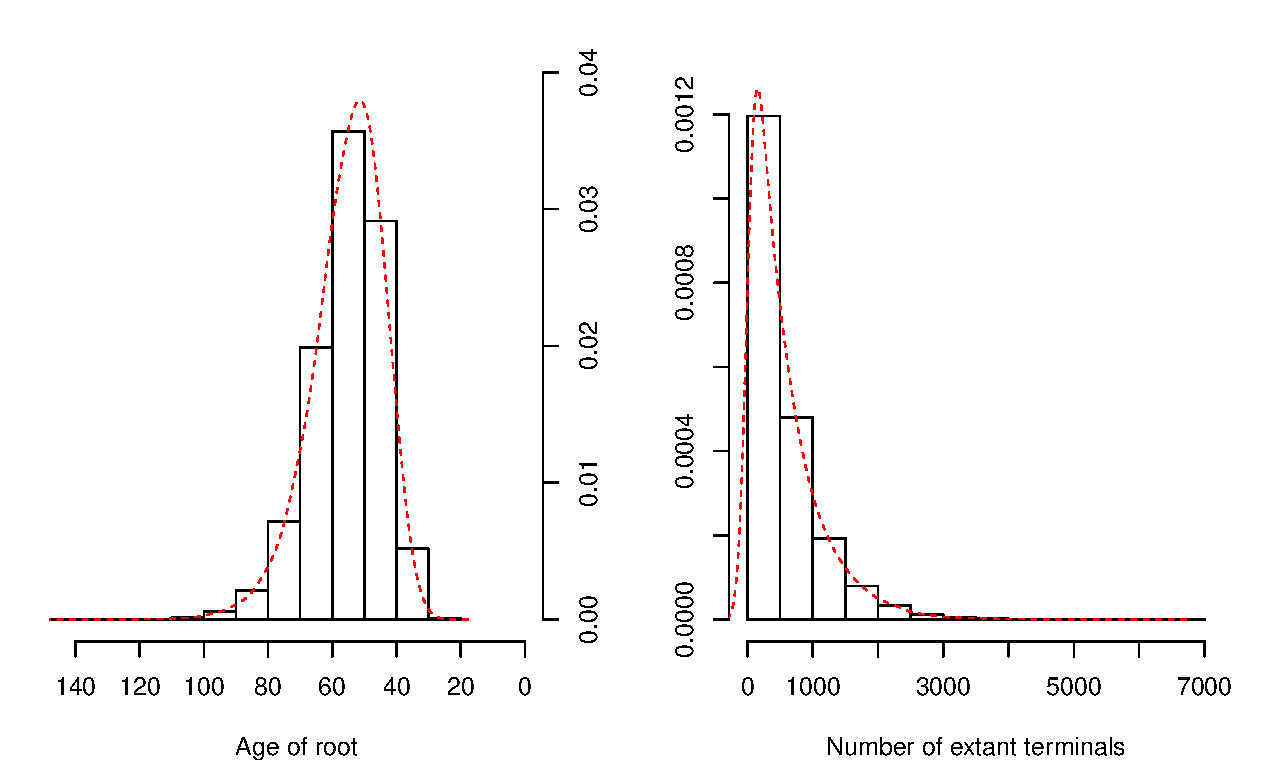
\includegraphics[width=86mm]{Fig1.eps}}
\caption{Parametric bootstrapping of a diversification process. The primate phylogeny of \cite{Springer2012} was fit to a birth-death model (pxbdfit). To explore the breadth of plausible diversification outcomes the maximum likelihood parameters (b: 0.339487, d: 0.268944) were used to simulate (pxbdsim) 25000 phylogenies conditioned on either the extant diversity (367, left) or root age (66.7066 Ma, right) of the empirical tree.}\label{fig:01}
\end{figure}


\section{Conclusion}

\texttt{phyx} was designed to complement existing phylogenetic toolkits by
enabling the exploration, manipulation, analysis, and simulation of
phylogenetic objects directly from the command line. Moreover, by conforming
to a stream-centric approach, memory requirements are reduced significantly so that large volumes of data can be processed on personal laptop
computers. \vspace*{-10pt}

\section*{Acknowledgements}

We thank Ya Yang and Jeff Johnson for helpful discussions and comments on the manuscript.\vspace*{-12pt}

\section*{Funding}

This work has been supported by the Caryophyllales grant and the AVATOL grant \textbf{STEPHEN IS PUTTING THIS TO MAKE SURE STEPHEN ADDS THESE!}\vspace*{-12pt}

\bibliographystyle{natbib}
%\bibliographystyle{achemnat}
%\bibliographystyle{plainnat}
%\bibliographystyle{abbrv}
%\bibliographystyle{bioinformatics}
%
%\bibliographystyle{plain}
\bibliography{document}

\end{document}
